%%% Thesis Introduction --------------------------------------------------
\chapter{INTRODUCTION}
\label{chap:intro}
\graphicspath{{Introduction/IntroductionFigs/EPS/}{Introduction/IntroductionFigs/}}
\nomenclature[z1]{\cms}{Character Motion Synthesis}
\nomenclature[z2]{\cpg}{Central Pattern Generator}
\nomenclature[z2]{\dof}{Degree of Freedom}

\section{The Challenge}
Character Motion Synthesis (\cms) research aims at generating motions for virtual characters.
It is a valuable topic for both industry and academic community. 
Besides major applications in the media industry, where both computer games and animation films depend heavily upon character motions for storytelling;  
CMS also has applications in many different areas, such as user interface design, psychology, sports and medicine.

The challenge of \cms research is not to make characters move, but how to make them lifelike. 
Underneath this challenge is human's marvellous ability of motion perception. 
In fact, motions are very similar; 
while from the varieties in motion details, humans can infer the changes in mental states, health conditions or the surrounding environment.
\note{uncanny valley}
A famous phenomon of motion perception characteristics is the ``uncanny valley''.
For characters with realistic humanlike appearance, slightly artefacts in motions may result a big drop in human likeness.



Nowadays in industry, high quality motions are mainly generated by manual work. 
In applications,characters are very complex and contain a large number of joints, making animation a tedious work.
Making it worse, reusing motion animation is also difficult and prone to artefacts.
High level animation tools are badly needed. 

\note{Do An introduction for physicall based animaiton?}
Physics based \cms is the current research endeavor.
The expectation is the elimination of the artefacts that violate physics laws and interactive dynamic responses to environmental perturbations.
Currently,this paradigm faces many difficulties including computational cost and modelling complexity.
Same problems are spotted by biological researchers from different perspectives.

The ``uncanny valley '' prompts us the percetion question of dynamics.
Motion is not judged by validity of physics.
Some awkward artefacts are spotted instantly even they are physically feasible, while many physical impossible motions are accepted as realistic and enjoyable. 

How we perceive the world is foudation how we move through it.
The oddity of motion perception and control suggests a different principle adopted by the neural system.
Difficulties in \cms reflects the inferiority of artificial control.
By exploring new biological research , this thesis proposes a different approach.

 

\section{Agile Animals}
%\note{Underlying these problems} is our misunderstanding of animal motions.
Although motions of animals have fascinated us for thousands of years, we still don't fullly understand how they move.
Animals are very different from artificial machines.
Investigations into such differences provide an in-depth understanding of problems of nowadays CMS researche.
%some basic questions of motor control and motion perception remain open. 
%And answers to such questions become even more valuable nowadays. 
%Advance in this topic will greatly influence the biology, robotic engineering even intelligent research.
\note{The difference between biological motor system}

%The paradoxes is even human are good at motor control and motion perception; human still don’t have an idea of how we move and how we perceive motion.
%Before going into details into the research ideas, we first review some puzzles troubles the foundation of CMS. 
\begin{itemize}
\HiItem {Degrees of freedom ({\dof}s)}.
From Mechanical perspective, animals have many more {\dof}s than their artificial counterparts.
An artificial ship can be approximated by a simple rigid body; while the flexible vertebrae of fishes has tens of {\dof}s.


In principle, the extra {\dof}s admit more types of motion variations. 
But from the control perspective, the extra {\dof}s complicate the control problem. 
For a human to take one step,  the neural system controls more than 600 muscles .
Extra {\dof}s are redundant and become the ``{\dof}s Curse'' for motor control.
 
\HiItem {Versatility}
Most artificial machines are designed with a single purpose.
While animals are capable  of unlimited motion tasks.
For human, beside the walking, swimming and many other styles of locomotion , human motion behaviour involves lots of tools, such as cars, skate, bicycle, and tennis.
Some behaviours negalected by \cms research the feeding, breeding, language, vision depends on motor control. 
Follows the question how much mental resource is allocatted for motor control.

It seems much following traditional control approach but biologicalresearch shows very little.

\HiItem{Performance}
Even for animals,  motor control is more complex , the motion results surpass artificial machines in many aspects.
Natural motion are more
\begin{enumerate} 

\HiItem{robust}
Human can maintain walking stability on tough terrain unaccessible for vehicles.

\HiItem{maneuverable and speedy}
Typical modern airplanes will travel $32\: body\: lengths/sec$ and yaw $720\: deg/sec$ at max.
while pigeons may travel $75 \:body\: length / sec$, yaw at about more than $5000deg/sec$.

\HiItem{Energy Efficient}
The energy consumed by human walking is only $5\%$ of that for the world famous humanoid ASIMO.
\end{enumerate}

\end{itemize}



%For computer animation research, the key principle is we should know the things we animate.
%Natural motion system has many valuable properties which are not captured by current motion synthesis methods.
%\begin{itemize} 
% \HiItem{robust}
%Natural motions are adaptive to the changes in the environment or body conditions. 
%A common example is human locomotion. 
%Walking on different terrains will exhibit different gait while the balance is maintained. 
%
%\HiItem{speedy}
%Some motions of animals are very fast, honey birds may vibrate their wings in kHz.
%The astonishment is to the speed of motion, more puzzling is that the neural system can solve the complex motion control problem in such a short time. 
%When an animal avoids obstacles at very high running speed, 
%it must continue its running, make a turning and keep balance at the same time. 
%It seems easy for the neural system to plan complicate motions.
%\HiItem{Energy Efficient}
%Natural Motions are energy efficient.
%In theory, this idea is supported by Darwin's Theory of Evolution.
%But animals spent far less energy than our expectation.
%An example is that the energy consumed by human walking is only 5\% of that for a robot of the same scale.
%\end{itemize}

\section{Motor Invariant Theory}

The approach proposed in this thesis is different from current \cms methods in many different ways .
A side by side comparison will highlight the distinction and novelity. 

\subsection{Major Differences}
\begin{itemize}
\HiItem {Control Function Model}
The procedure approach support computational model of motor control.
It is the redundant {\dof}s that spoil this approach  with inhibitive computational cost.
Pure procedures methods are impossible to run in real-time.

As an alternative, some researchers support the memory based model for motor control and have developed data-driven methods.
But such methods lacks the versatility and adaptivity.
Unlimited memory for data is needed and searching in ever increasing database becomes more and more challenging.

My idea of is different from the two above.
The foudation idea of the new approach is that motions are ``easy'' and need little control effort.
It is the body and environment that play the crucial role, their dynamic interaction form the basic templates for motor control.
the neural system only tweaks the basic templates for specific purpose.



 
 
	
\HiItem{Control Strategy}
Most artificial control method follows the principle of feedback.
The motion trajectory is planned first and control is applied to counteract perturbations.
This method is also called ``continuous shooting''.


The control strategy of new approach is feed forward.
The principle control idea is making motions ``easier''.
If perturbations can be predicted, measures are taken beforehand to prevent ``failure''.
Thus motion trajectory is unconcerned, only the final result matters.


\HiItem{Natural Dynamics} 
Many \cms research plan the motion trajectory before execution.
The natural dynamics of the body and environment is treated as perturbations which are canceled by control input.


The mechanical structures of animals have evolved with the enivronment for millions of years, in the process of natural selection.
They are advantages rather than hanicap. 
The new approach limit the control input and explore the natural dynamics for the natural-looking features.
\end{itemize}


\subsection{Motor Invariant Theory}
%In this thesis, we propose different idea towards motor control and motion synthesis.
%In this research, we propose a different motion synthesis method based on a different motor control theory.
%
%An insightful discovery is that motor control can be “easy”.
%For some situation, some tasks mainly explore the properties of the body and environment and can be achieved with little control effort.
%In nature, we don’t finish difficult motion tasks, we select many easy motion tasks that we are good at, connect or modify them for our special purpose.
%
%The “easy” tasks are called motion primitives; they are the basic elements of our motor ability. 
%When we modify the motion primitives, some valuable properties of motion primitives are kept unchanged, and the maintained properties are called motor invariants.
%
%The inspiration of our idea comes from related biological research, which covers biomechanics and neural science.
To make new ideas workable, new mathematical tools are introduced to develope control techniques.
At the center of the new theory is the mathematical modelling of the motion templates and the ``tweaking'' exerted by the neural system.
The insightful discovery is that when motion adapts, some properties are maintained, thus called motor invariants.
Based on this idea, we established a theory of motor control, the motor invariant theory.


Qualitatively, the property of ``easiness'' should be maintained.
Structural Stability arise as an abstraction of the intuitive idea of ``easiness'' of motor control.
Motion adaptations are modelled as topological conjugations. 

For the quantitative properties, we explore the idea of ``Symmetry''.
Lie Groups are introduced to modeling the ``tweaking'' actions that maintain the local quantative properties.


More complex tasks are executed by combining simple tasks together,just like we connecting alphabets into meaningful sentence.
The basic motion tasks are called motion primitives, of which the number is limited.
For an animal, the repetorie of motion primitives is determined by the body and environment.


Although new mathematical tools seems abstruse at first glimpse.
The ideas behind are simple and illustrative, and can be explained well by daily phenomenon



\subsection{Floating Ships}
We use the floating ships as an example to show the relation between ``easiness'' of motor control and how the topological conjugacy comes into the theory of motion.
In real life, ships floating on the wavery water, some of which the height is much larger than width,as shown in Figure~\ref{fig:ShipFloating}.

The interesting question how the ship maintain its posture.
Through analyzing the qualitative dynamic properties, we conclude that maintaining posture is a trival task.
And our conclusion applies to different ships for their dynamics are topological equivalent.


\begin{figure}[!htbp]
  \begin{center}
    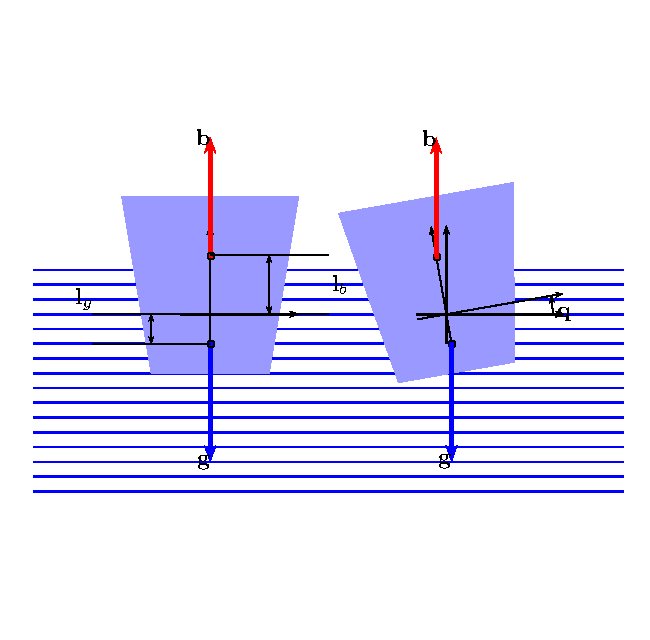
\includegraphics{ShipExample}
    \caption{The Floating Ship Example}
    \label{fig:ShipFloating}
  \end{center}
\end{figure}

\subsubsection*{Dynamics}
The sway motion shown in Figure ~\ref{fig:ShipFloating} is described by Equation~\ref{eq:shipflow}
\begin{equation}
\label{eq:shipflow}
I_{e}\ddot{q}+d\dot{q}=T_{G}+T_{B}+T_{F}=(Gl_{g}-Bl_{b})sin(q)+T_{F}
\end{equation}

$q$ is the swaying angle.
$I_{netia}$ is the inertia,  
$d$ is the damping coefficient,
$T_{G}$ is the torque of gravity, and $T_{B}$ is the torque of buoyancy.
$T_{F}$ is the external control torque.

when $T_{F}=0$, no control effort is applied, the floating ship becomes an \emph{autonomous system} and is governed by natural dynamics.





\subsubsection*{Equilibrium Posture}
Ship will only rest at postures when $T_{G}+T_{B}+T_{F}=0$.
Only two postures qualified are called \emph{Equlibrium} Postures, show in Figure ~\ref{fig:ShipEqulibrium}
\begin{figure}[!htbp]
  \begin{center}
      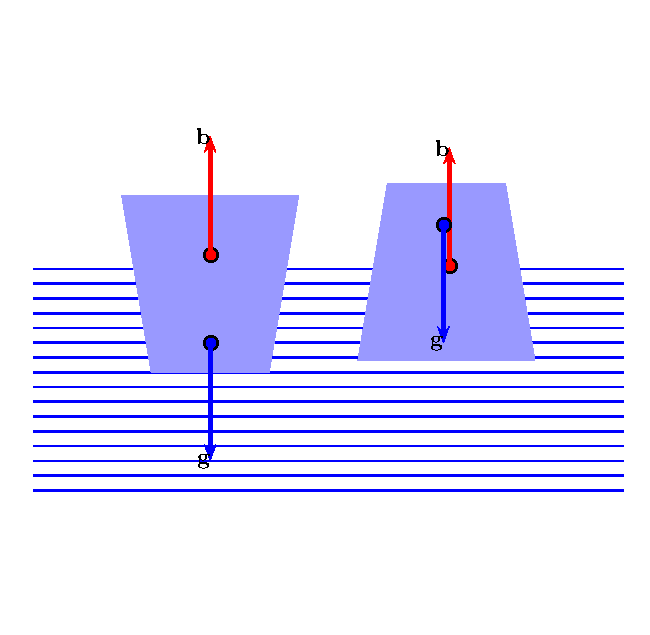
\includegraphics{ShipEquilibrium}
    \caption{Two Equilibrium Postures}
    \label{fig:ShipEqulibrium}
  \end{center}
\end{figure}



The two postures are qualitative different. 
Such differences are illustrated with the \emph{phase plot}.
On phase plot, horizontal axis represents the sway angle $q$; the vertical  axis  the angle velocity $\qd$. 
The movement of the ship are shown as a curve.

The left posture is \emph{attractive} or \emph{stable}.
If a small perturbation moves the ship away from the left posture, it will return to the equilibrium posture automatically as shown in Figure~\ref{fig:StablePosture}.

The right posture is \emph{repelling} or \emph{unstable}.
If a small perturbation moves the state of the ship away from the equilibrium posture, it will move away from the posture, as shown in Figure~\ref{fig:unStablePosture}.

 
\begin{figure}[!htbp]
  \begin{center}
      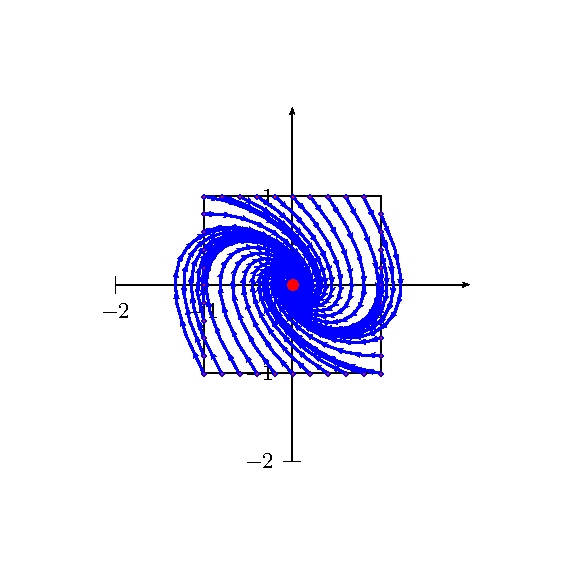
\includegraphics{stablePosition}
    \caption{Stable Posture.Start from a position nearby, the ship will automatically move toward the attractive posture}
    \label{fig:StablePosture}
  \end{center}
\end{figure}


\begin{figure}[!htbp]
  \begin{center}
      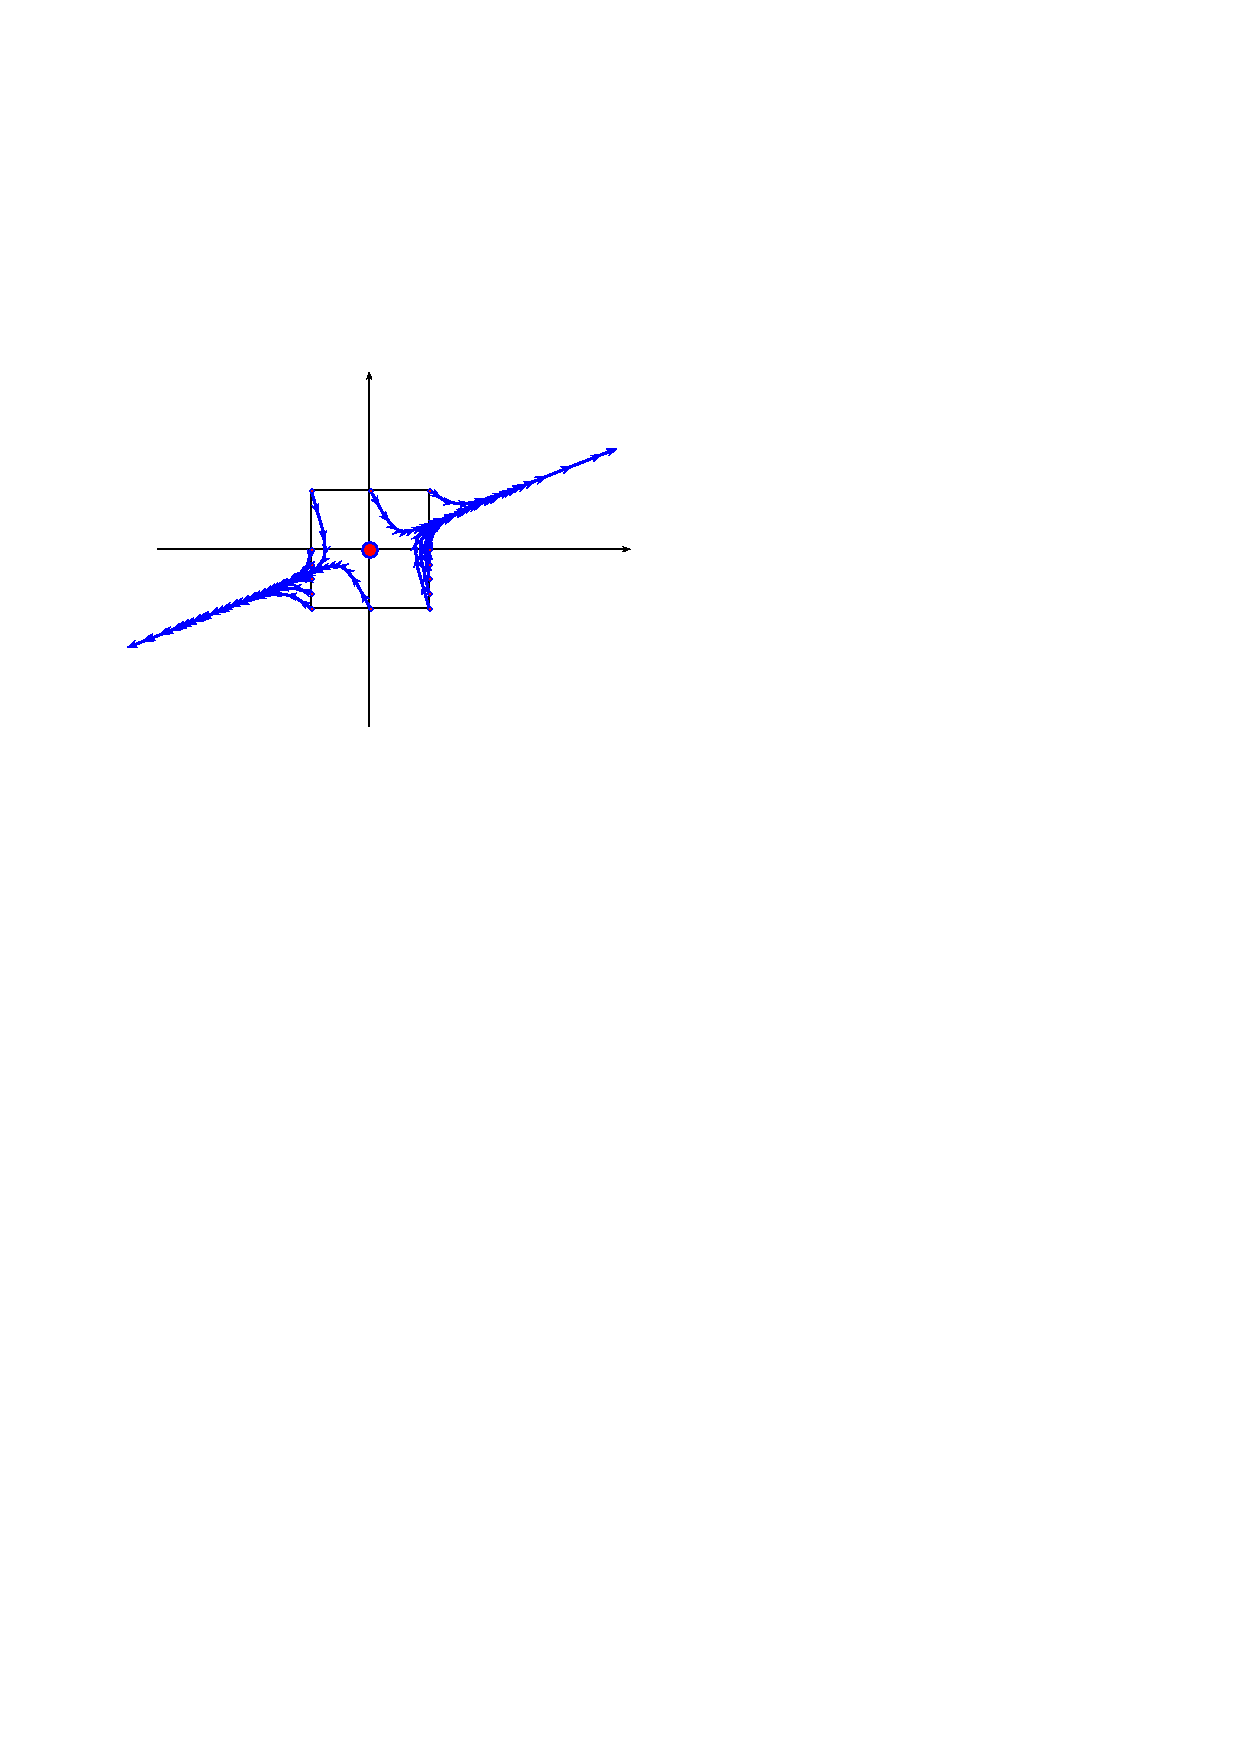
\includegraphics{unstablePosition}
    \caption{Unstable Posture. Start from a position nearby, the ship will move automatically away from the repelling posture}
    \label{fig:unStablePosture}
  \end{center}
\end{figure}


\subsubsection*{``Easiness''}
All the possible motion curves form the \emph{phase portrait} of floating system system. 
The discovery is that all the curves will move away from the repelling posture to the attractive posture.
This means the floating ship can maintain the left posture automatically without any control.
Several curves are show in Figure ~\ref{fig:globalflow}

\begin{figure}[!htbp]
  \begin{center}
   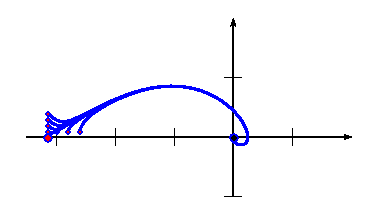
\includegraphics[width=0.7\textwidth]{ShipGlobalFlow}
   \caption{Global Properties of the Motion Curves: All the curves move aways from the repelling posture(Red) towards the attractive one(Blue)}
   \label{fig:globalflow}
  \end{center}
\end{figure}

Thus  the conclusion is  maintaining the left posture is trival. 
Structure Desing (the center of bouyancy is above the center of gravity) provides the ship with excelent balancing ablity.


\subsubsection*{Generalization of the Ship Example} 
The conclusion is independent of the design detail of the size, weight of the ship. 
Same way will result in different sway motions for different ships.
As long as the qualitative properties (the centre of buoyancy is above the centre of gravity) is maintained, balancing is ``easy''.
For a different perspective,   we conclude ship will adapt it balancing motion when design parameters are changed.


In the geometrical perspective, the phase portraits of all the ships share some properties:
\begin{itemize}
\item one repealing point 
\item one attractive point 
\item all motion curves move away the repelling point to the attractive point. 
\end{itemize}


\begin{figure}[!htbp]
  \begin{center}
   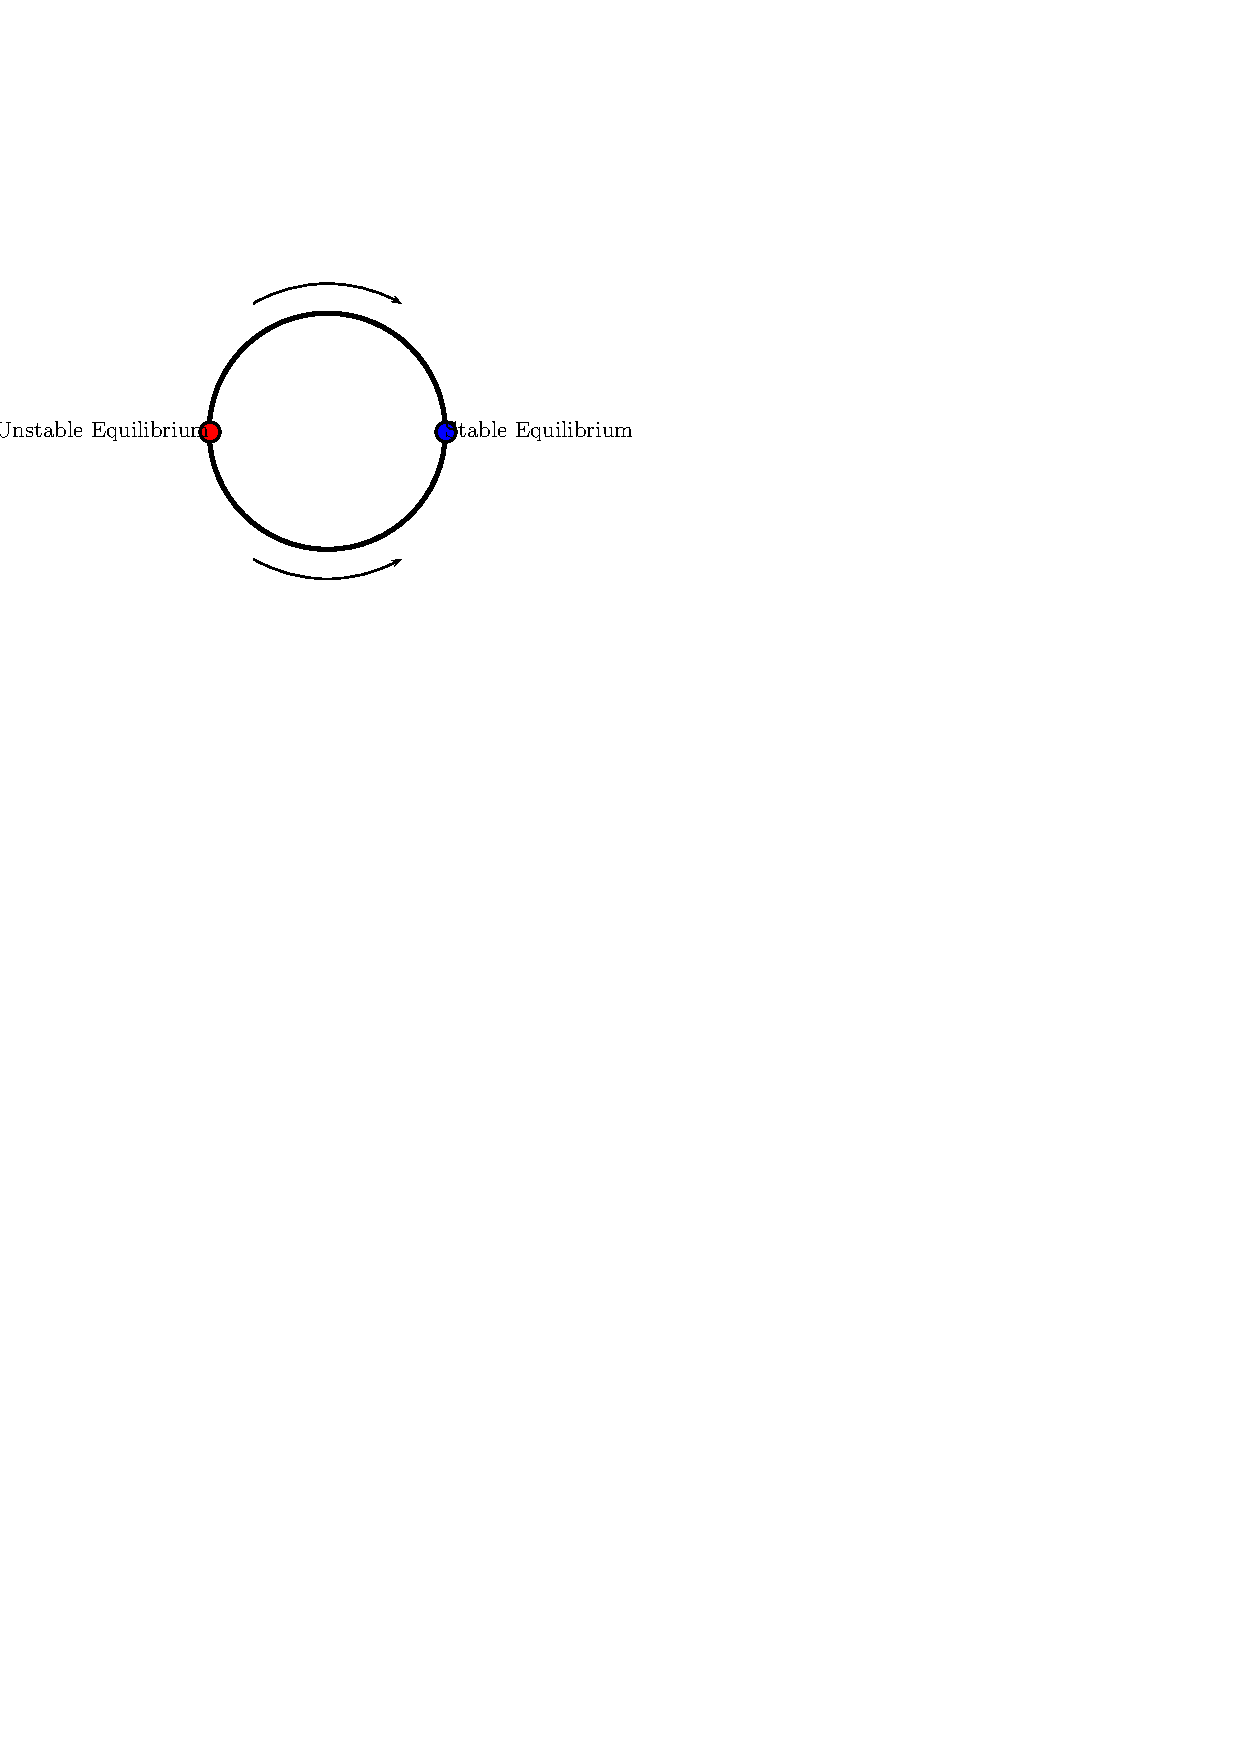
\includegraphics{topologyStructure}
   \caption{all the ship share the same topological structure.}
   \label{fig:topologyStructure}
  \end{center}
\end{figure}

The common properties of different ships are represented by Figure~\ref{fig:topologyStructure}.
Such properties are “topological property”.
As long as the topological structure is preserved, maintaining posture is ``easy''.

For dynamic systems of two ships are described by two equation $\dot{\state}=F_1(\state)$ and $\dot{\state}=F_2(\state)$.
Sharing the same topology means they are topological equivalennt $F_1 \simeq F_2$, or more specifically \emph{topology conjugacy}.
$F_1$ and $F_2$ are called \emph{analogous systems}.


In our motion synthesis framework, the topology is one motor inviarant. the \emph{global motor invariant}.
Global motor invariant encapsulates the qualitative properties of a dynamic motion.
Motion adaptations that come from the parameters of the dynamic system are called \emph{System Adaptation}


\subsection{The Mass Spring System}
Even the body is complex,human can finish motion tasks with high accuracy instantly, which propose the puzzle how neural system achieve this.
The idea we propose  is that for natural animals,  new motons are not synthesized by solving the  motion dynamics directly, they are the transformed version of the some motion templates.
 This idea can be  illstruted by the following mass spring example

\subsubsection*{Dynamics}
\begin{figure}[!htbp]
  \begin{center}
    \includegraphics[width=0.7\textwidth]{MassSpring}
    \caption{the mass spring system:$q$ is offset from the rest length}
    \label{fig:massspring}
  \end{center}
\end{figure}


Although simple, the mass spring system in Figure~\ref{fig:massspring} captures some of the important properties of motor control system.
The biological motor muscle actuation works more can be modelled as spring and bones can be simplified as mass.
The canonical equation of mass spring system is Equation~\ref{eq:mass-spring}

\begin{equation}
\label{eq:mass-spring}
\ddot{q}+q=0.
\end{equation}

In a similar manner,  the phase plot of the mass spring system is shown in Figure~\ref{fig:massSpringPhasePlot}


\begin{figure}[!htbp]
  \begin{center}
      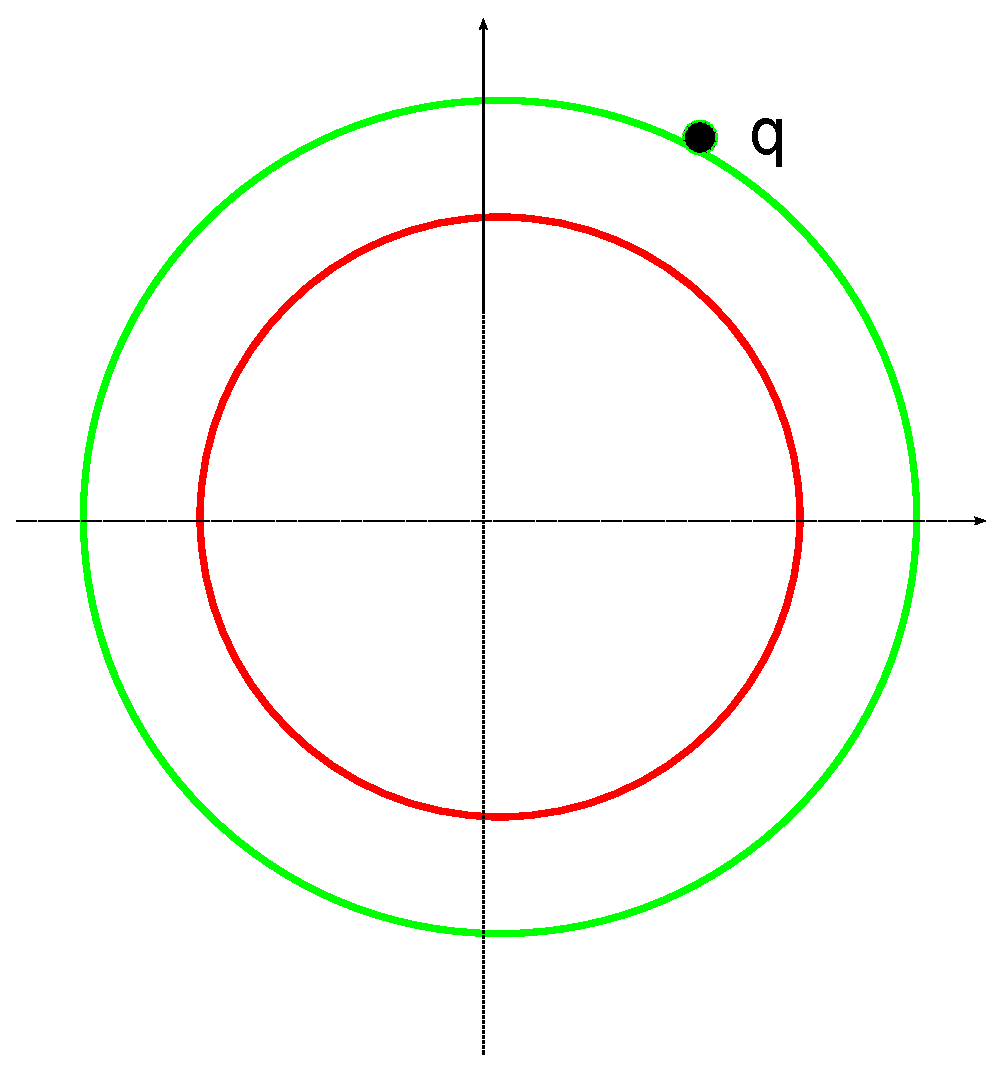
\includegraphics[width=0.5\textwidth]{MassSpringPhasePlot}
    \caption{Mass Spring Phase Plot:two motion curves are shown.The red one and the green pass through different state $\state$,$\state^{'}$}
    \label{fig:massSpringPhasePlot}
  \end{center}
\end{figure}

\subsubsection*{Symmetry and Transformation}
Even it is simple, it is highly unlikely we plane the motion by solving Equation~\ref{fig:massSpringPhasePlot}
For the mass spring system,different motios can be gained through transformation.
Given a state $\state^{'}=[q,\qd]$, it is on the green circle that shares the centre with the red one, but has a bigger radius, the green curve is a scale red curve.
The property that we can transform one motion into another is because we massspring system have the property called ''symmetry''.
In fact we can ignore the complexity of the dynamic system, as long as we know the ``symmetry'' property of a dynamic system. 
Provided with one motion, we can work out all the possible motions.

\subsubsection*{Dynamic Perception}

The dynamic system can be encoded in a different manner,a possible way is store one motion curve and the symmetry property of the dynamic system.
Impact of this idea for motor control is far reaching in several ways. 
Besides reduction of the computational costs, it also provides us with an alternative idea for motion perception. 
We don't varify the motion believability by solving motion equations; we check the ``symmetry'' property of the motion.
If we can transformed the observed motion(green) into our memorized motions (red), than we think the motion are realistic, otherwise we detect artefacts.


\subsubsection*{Local Motor Invariant and Transform Adaption}
To varify the symmetry properties of motion, it is unnecessary to work out the transformation directly. 
Some property are kept invariant transformations, for the mass spring system example, the ``shape'' is kept during scale transformation. 
From Differential Geometrical perspective,  the curvature is invariant. 
From mechanical view, we can say for each motion, the energy is kept along the curve, and different motion is of different levels of energy. 

Properties of energy and curvature are called \emph{Local Invariant}. 
And the transformation from one motion to another is called \emph{transform adaptation}.

\section{Contribution}
\emph{Global Motor Invariant} captures the qualitative properties while \emph{Local Motor Invariant} determines quantitative properties. 
For our motion synthesis, controllers are designed to preserve the both motor invariants. 

Motion Adaptation is achieved through \emph{System Adaptation}(change system parameters) and \emph{Transform Adaptation}.

Compared with current \cms methods.
\begin{enumerate}
\item More sytle of motion adaptation are generated.Compared with traditional dynamics \cms methods,\emph{System Adaptation} and \emph{Transform Adaptation} generate more types of adaptions in motion style.
\item Userbility are better, \emph{Transform Adaptation} provides a easy method for adapt motion. Artists can generate complex dynamic motion adaptation by simply adjust one parameters.
\item It is more computational efficient. Our motion synthesis can generate motions in realtime.
\end{enumerate}

For the method is based on the bioligical motor control research, but for the application purpose, we adopted a different research paradigm.
Currently, emprical statics are the main paradigms for develop new biological theory.
The mathematical tools we developed and introduced are alternatives to the emprical statistics.
They may shed light into some biological questions, can be treated as theorical candidates for further biological research.

\begin{enumerate}
\item Motion Primitive is an old idea in biological research, while currently method for identy motion primitives are based on empirical statisics and machine learning.
The theory we present is based on rigid mathematical analysis.
Besides identifification of  motion primitives, it also answer the why question and many implication and deduction can be implied.

\item Some neural structures such as \cpg , their functions on motor conrol are well agreed, while a concrete mathematical model how the \cpg adjust motion is still lacking.
In our research, we develop the method for adjust \cpg parameters to ``tweaking'' motion. 

\item For perception research, motion and dynamic proception mechanism of neural system is still unclear.
The motor invariant theory provides computational efficient and workable mathematical machinery for encoding motion and dynamics.

\item Synergy in muscle actuation is identify by emprical methods. The `` control symmetry '' method we introduced can treated an mathematical theory for explain  ``synergy''.
\end{enumerate}







\section{Organization of the Thesis}

This thesis is organized as follows.
 
In Chapter~\ref{chap:background}, previous research work of motion synthesis and biological motor control are discussed, which are the motivation and justification of our ideas.
 
In Chapter~\ref{chap:gi}, \emph{Global Motor Invariant} and qualitative property of motion are discussed. 
Differential topology are introduced to analyzing the qualitative properties of motion.
Bilogical based  method for maintaining the global motor invariant are developed.

In Chapter~\ref{chap:li}, the idea of Local Motor Invariant and Symmetry is the focus.
Lie Group are introduced for analyzing and develope control method to preserving symmetry. 


In Chapter~\ref{chap:msf}, we discuss the combinations of ideas.
for each motion primitive, we develop the strategy for makeing global and local motor invairant controller work in harmony.
Motion primitives transition is dicussed and the theory for how to combine simple motion elements into more complex motion.
The animation system, we also talk about the software archetecture and work flow for applying the new method for generating animations.

Chapter~\ref{chap:gi},~\ref{chap:li},~\ref{chap:msf} lay the theory foundation for the motion synthesis control and be treated as the Motion Invariant Theory.
Following chapters focuns on application of this theory for generating different motions.



In Chapter~\ref{chap:walk}, we focus on synthesizing motion of one primitive, bipedal walking,which is one of the most interesting and challenging  in motion synthesis research.
We show how our method main the stability and generating adaptive gaits for different scenario.


In Chapter~\ref{chap:stance}, combination of motion primitives are discussed.
A new Motion Primitive (the balancing) is developed. 
Primitives transition motions are generated for stance to walk and walk to stance transitions.

In Chapter~\ref{chap:highdor}, we discuss about extend the basic idea to more complex characters and dynamic systems.
Three different strategy are developed for different situations.

In Chapter~\ref{chap:Conclusiont}, we conclude our discussion comparative advantages of research and future work.
After a retrospection, we proposed some new question and ideas for graphics and neural science for further research.





%%% ----------------------------------------------------------------------


%%% Local Variables: 
%%% mode: latex
%%% TeX-master: "../thesis"
%%% End: 

